\section{Border-Collision}
\setauthor{Fabian Maar}

Um den Benutzern und Benutzerinnen ein möglichst realistisches Gefühl für die Ausstellung zu geben, ist es wichtig, den Ausstellungsraum auch so zu gestalten. Daher ist der Raum durch Wände abgegrenzt, wodurch es nicht mehr möglich ist, sich über den Raum hinaus zu bewegen. 
Um eine Kollision mit der Wand zu berechnen, gibt es durch die Three.js Bibliothek einige Möglichkeiten.
\subsection{Erster Ansatz}
Eine davon ist, eine Bounding Box zu erstellen. Dabei unterscheidet man zwischen zwei verschiedenen Arten. Zum einen verwendet man die Axis Aligned Bounding Box, um eine Box rund um das 3D-Objekt zu erstellen, die sich nicht an die Rotation des Objekts anpasst. Die zweite Variante ist die Oriented Bounding Box, die im Endeffekt gleich funktioniert, sich aber darin unterscheidet, dass sie sich an die Achsen des Objekts anpasst. Da sich die Bounding Boxen jedoch über das ganze 3D-Objekt erstrecken, wird eine Kollision direkt berechnet, nachdem der*die Benutzer*in den Raum betritt. Da sich die Bounding Boxen nicht an jede einzelne Wand anpassen konnten, musste ein anderer Lösungsweg gefunden werden.

\begin{figure}
    \centering
    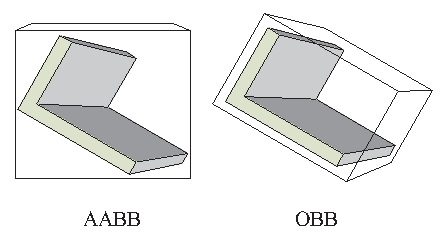
\includegraphics[scale=0.65]{pics/aabb_obb.png}
    \caption{Der Unterschied zwischen AABB und OBB}
    \label{fig:impl:aabb_obb}
\end{figure}

\subsection{Zweiter Ansatz}
Um eine Veränderung der Position des*der Benutzers*in festzustellen, muss die Veränderung der Kameraposition evaluiert werden. Dabei wird beim initialisieren der Kamera eine Kopie von ihr erstellt. In der Animate-Funktion wird eine Veränderung der Kamera überprüft, indem die Positionen der Kamera mit der Kopie verglichen werden. Die Kamera nimmt dabei immer eine neue Position ein, wenn sich der*die Benutzer*in im Raum bewegt, während die Kopie dabei die alte Position der Kamera einnimmt.    
Jedesmal wenn eine Veränderung geschieht, wird überprüft, ob die Kamera mit der Wand kollidiert. Dies geschieht, indem ein Raycast mit den Positionen der Kamera und der Kopie initialisiert wird. 
\subsection{Far und Near}
Die Attribute Far und Near werden dafür verwendet, um die Objekte, die im Ray liegen, einzugrenzen. Dabei können die Werte nicht negativ sein und der Far-Wert muss größer als der Near-Wert sein. Um die Kollision erst direkt am Ursprungsort, im Falle der Kamera, des Rays zu berechnen, wird der Far-Wert auf 100 gesetzt.
   	
Nachdem der Raycast korrekt initialisiert und angewandt wurde, muss bei einer Berührung mit der Wand nur noch richtig damit umgegangen werden. Dabei wird die Bewegung des Benutzers gestoppt. Um diese auch wieder zu starten, muss sich der*die Benutzer*in weg von der Wand begeben. Überprüft wird dies nach jeder Benutzer*inneneingabe mit einem Event-Listener. Falls nach dieser keine Berührung mehr mit einer Wand besteht, wird die Bewegung fortgesetzt und der*die Besucher*in kann sich wieder frei im Raum bewegen.
\newpage

